\chapter{Implementatie}

\section{Selectie van de DBMS's}

\subsection{Selectiecriteria voor DBMS's}
Bij de selectie van de systemen of een systeem een bepaalde eigenschap al dan niet ondersteunt. In het totaal zijn er 5 verschillende eigenschappen waarop wordt geselecteerd. 

\paragraph{Vrije software} Om testen tussen verschillende DBMS's te kunnen vergelijken op een gelijkaardige infrastructuur, is het nodig dat deze software kan geïnstalleerd worden op de eigen infrastructuur. Daarnaast is er in dit onderzoek gekozen voor gratis beschikbare software. 

\paragraph{Persistentie} Voor het testen van de beschikbaarheid van de data, is het een voordeel dat de data op harde schijf aanwezig is: bij herstel dient er minder data over het netwerk gestuurd te worden. Om deze reden hebben deze systemen een voorkeur op systemen die de data enkel in geheugen houden. 

\paragraph{Replicatie} Eén van de testen is de beschikbaarheidstest, indien de data maar op een enkele server opgeslagen is, zal de data op de uitgeschakelde server niet langer beschikbaar zijn. Met replicatie zal de data op verschillende servers opgeslagen worden en zal de data nog steeds beschikbaar zijn in het geval van een enkele uitgeschakelde server. 

\paragraph{Data distributie} Het is de bedoeling om systemen te testen die een grote hoeveelheid data kunnen opslaan. Om aan deze vereiste te voldoen, is het nodig dat elke server niet al de data opslaat bij een voldoende hoog aantal servers (bij weinig servers, is elke server nodig om aan de replicatie vereiste te voldoen)

\paragraph{Ondersteuning voor verschillende query methodes} Bij de testen worden er 5 soorten queries uitgevoerd: invoegen, aanpassen, verwijderen en opvragen van een individueel record en het opvragen van meerdere queries. De DBMS moet ondersteuning voor deze queries. De eerste 4 kunnen in al de systemen geïmplementeerd worden met één of meerdere queries. Maar het opvragen van meerdere queries is in bepaalde systemen niet mogelijk en deze worden om deze reden niet behandeld. 

Voor elk van de systemen besproken in sectie \ref{sec:BesprekingDBMS}, is het eerste criterium voldaan voor al deze systemen. De overige 4 criteria zijn samengevat in tabel \ref{table:vergelijkingNosql}. Naast de 4 criteria, is er gekozen om systemen van verschillende klassen te hebben met uitzondering van Key-Value. Samen met mijn collega Arnaud Schoonjans \cite{thesisArnaud}, zijn er in verschillende systemen verder onderzocht. In deze thesis zijn  HBase, MongoDB en Pgpool-II verder onderzocht, in de thesis van mijn collega zijn Cassandra, Apache CouchDB, Riak en MySQL verder onderzocht.  
 
\todo{Update table :-)}
\begin{table}
    \begin{tabular}{lll|l|l|l|l|l|l|l|l|l}
    ~                & ~         & \multicolumn{2}{l}{ \rotatebox[origin=c]{90}{Column database}} & \multicolumn{2}{l}{\rotatebox[origin=c]{90}{Document database}} & \multicolumn{4}{l}{\rotatebox[origin=c]{90}{Key-Value database}} & \multicolumn{2}{l}{\rotatebox[origin=c]{90}{Relationele database}} \\
    ~                & ~         & \rotatebox[origin=c]{90}{Cassandra} & \rotatebox[origin=c]{90}{HBase} & \rotatebox[origin=c]{90}{Apache CouchDB} & \rotatebox[origin=c]{90}{MongoDB} & \rotatebox[origin=c]{90}{Lightcloud (Tokyo)} & \rotatebox[origin=c]{90}{Memcache} & \rotatebox[origin=c]{90}{Riak} & \rotatebox[origin=c]{90}{Voldemort} & \rotatebox[origin=c]{90}{MySQL} & \rotatebox[origin=c]{90}{Pgpool-II (PostgreSQL)} \\
    \multicolumn{2}{l}{Persistentie} & ~               & ~     & ~                 & ~       & ~                  & ~        & ~    & ~         & ~                    & ~                      \\
    \multicolumn{2}{l}{Replicatie} & ~               & ~     & ~                 & ~       & ~                  & ~        & ~    & ~         & ~                    & ~                      \\
    \multicolumn{2}{l}{Data distributie} & ~               & ~     & ~                 & ~       & ~                  & ~        & ~    & ~         & ~                    & ~                      \\
    Query soort      & Aanpassen & ~               & ~     & ~                 & ~       & ~                  & ~        & ~    & ~         & ~                    & ~                      \\
    ~                & Range     & ~               & ~     & ~                 & ~       & ~                  & ~        & ~    & ~         & ~                    & ~                      \\
    \end{tabular}
    \caption{Ondersteuning van de besproken DBMS's naar de selectie criteria met de gekozen systemen geaccentueerd.}
    \label{table:vergelijkingNosql}
\end{table}


\section{Gedetailleerde bespreking van de geselecteerde DBMS's}
In dit gedeelte zal elk geselecteerd systemen in meer detail uitgelegd worden, met een focus op de systeem structuur. Een gemeenschappelijk element bij al deze systemen is dat niet alle noden dezelfde functie hebben, in andere DBMS's hebben allen dezelfde taak wat de installatie kan vereenvoudigen. 

Voor elk van de geselecteerde systemen zal de aangeboden API besproken worden met een blik op de datastructuur, daarna zal de systeem architectuur besproken worden. 

\subsection{HBase}

\subsubsection{Data structuur}
De data in HBase is gestructureerd in tabellen, die aangemaakt worden door middel van de API. Op het moment van aanmaak wordt er een schema van de tabel gemaakt. Voor elke tabel kunnen de kolommen meegegeven worden samen met een \textit{kolom familie} voor elke kolom, maar de kolommen kunnen ook gespecificeerd worden bij het schrijven van data. De gegevens per \textit{kolom familie} hebben dezelfde prefix en zullen fysisch samen opgeslagen worden. Indien verschillende kolommen tegelijk worden gelezen of geschreven, is het aangeraden om deze dezelfde \textit{kolom familie} te geven. 

De operaties beschikbaar in dit systeem zijn: get (verkrijgen), put (invoegen), scan (range) en delete (verwijderen). Het aanpassen van gegevens wordt uitgevoerd via een get waarbij een enkele kolom waarde van een record kan aanpast worden. Daarnaast zal er bij een scan een optimalisatie gedaan worden naar de cache grootte. Doordat er geweten is hoe groot een record ongeveer is in zijn geheel én hoeveel records er opgevraagd worden, kan de cache grootte berekend worden zodat er maar een enkele datacommunicatie nodig is. 

\subsubsection{Architectuur}
De gedistribueerde versie van HBase\cite{george2011hbase} is afhankelijk van 2 andere software systemen, namelijk Zookeeper\cite{hunt2010zookeeper} en Hadoop\cite{borthakur2007hadoop}, en volgt hiermee de structuur van Google's BigTable\cite{chang2008bigtable} die op zijn beurt afhankelijk is van Chubby\cite{burrows2006chubby} en Google File System\cite{ghemawat2003google}. Een overzicht van de architectuur bevindt zich in figuur \ref{fig:Hbase-structure}. Deze 3 systemen zullen kort besproken worden, van Hadoop tot Zookeeper en HBase. 

\begin{figure}[h!]
\centering
\includegraphics[width=\linewidth]{img/Hbase-structure.png}
\caption{Volledige systeemarchitectuur van HBase met Hadoop en Zookeeper. Bron \cite{ChinHBaseComprehensive}}
\label{fig:Hbase-structure}
\end{figure}

\paragraph{Hadoop\cite{borthakur2007hadoop}} HBase maakt gebruik van het Hadoop Distributed File System \gls{HDFS}, een gedistribueerd file systeem ontworpen om te werken op commodity hardware met een hoge fout tolerantie. \gls{HDFS} heeft een master/slave architectuur en bestaat uit een enkele \textbf{namenode}, de master server, die de naamruimte en toegangscontrole onderhoudt, en \textbf{datanode}s. De data wordt opgedeeld in blokken die in een verzameling van datanodes wordt opgeslagen, op deze manier is er data distributie en asynchrone replicatie. Deze master/slave configuratie zijn verschillende soorten van services en dient door de gebruiker zelf geconfigureerd te worden. \\
In de configuratie die hier gebruikt wordt, is \gls{HDFS} de methode de data in op te slaan in HBase met automatische replicatie en data distributie. Er is ook nog ondersteuning om dit lokaal op de harde schijf te doen bij een niet distribueerde installatie en om dit weg te schrijven naar S3.\cite{george2011hbase}

\paragraph{Zookeeper\cite{hunt2010zookeeper}} Zookeeper is een service voor het coördineren van gedistribueerde applicatie processen, met deze service biedt primitieven aan om synchronisatie, configuratie onderhoud en groepen en benaming te doen. Zookeeper is op zijn beurt een gedistribueerd master/slave systeem dat ontworpen is om snel te zijn bij dominantie van leesoperaties. De master/slave \\
HBase gebruikt Zookeeper onder andere voor het bijhouden van de status van regio server en hun locatie. \cite{george2011hbase}

\paragraph{HBase\cite{george2011hbase}} HBase is een master/slave systeem welke bestaat uit een HMaster en een HRegionServer. De \textbf{HMaster} is verbonden met Zookeeper en houdt op deze manier de status van de HRegionServers in het oog. Daarnaast is deze ook verantwoordelijk voor het opsplitsen van data (sharding) over verschillende regio's indien een tabel groeit en het toewijzen van een regio aan een HRegionServer.\\
De andere soort, \textbf{HRegionServer}s, is verantwoordelijke voor het dienen en beheren van regio's. Een regio is een deel van een tabel met daarin de feitelijke data die opgeslagen is in verschillende datanodes. Een HRegionServer zal de strikte consistentie afdwingen in HBase, dit kan doordat een enkele server verantwoordelijk is voor het uitvoeren van de data-updates. 

Dit is de globale structuur van het HBase systeem, in het totaal zijn er 5 verschillende soorten systemen, 2 bij Hadoop, 1 bij Zookeeper en 2 bij HBase. Enkele van deze systemen worden best gegroepeerd: de namenode wordt samengesteld met HMaster en een datanode met HRegionServer. Zeker deze laatste heeft een extra performantie invloed: HBase detecteert dat er lokale opslag van de data is en de regio zal steeds deze lokale opslag hebben. Dit gecombineerd met de asynchrone replicatie, zorgt ervoor dat het schrijven van data maar naar een enkele server gestuurd moet worden. 

De configuratie van de verschillende systemen gebeurt door middel van configuratiebestanden voor elke service waarna de volledige configuratie door het systeem zelf wordt gedaan, uitgezonderd het aanmaken van een tabel welke door de API wordt opgezet. 

\subsection{MongoDB\cite{mongodb-manual}}

\subsubsection{Datastructuur}
De data in MongoDB is opgeslagen in een database, die op zijn beurt een collectie bevat. Een database en collectie moeten niet aangemaakt worden op voorhand maar kunnen worden aangemaakt bij het wegschrijven van data. Een record is in un benaming een document en kan verschillende soorten velden hebben. Er zijn uitgebreide query mogelijkheden om data in te voegen, aan te passen, te verwijderen of een range aan te maken. Er is ook ondersteuning voor MapReduce\cite{dean2008mapreduce}. 

Bij het schrijven van data, kunnen verschillende eisen gesteld worden voor het voltooien van de actie, startende met de actie is over het netwerk verstuurd, de primary heeft de data geschreven tot een meerderheid van de secundaries heeft de data weg geschreven. \\ Bij het lezen kan men kiezen om de data te lezen van de primary, secundary of de dichtstbijzijnde node. Afhankelijk van de gekozen acties, kan er verondersteld worden dat er een verschillende consistentie garantie zal zijn.

\subsubsection{Architectuur}
MongoDB is een DBMS dat de vereisten van replicatie en data distributie op een gelaagde manier garandeert. In eerste instantie zal deze de replicatie vereisten invullen, daarna zal hierop horizontale schaalbaarheid ondersteund worden. 

\begin{figure}[h!] 
\centering
	\subfigure[Drie leden van een replica set met een primary en 2 secundaries. ]{\label{fig:mongodb-replicaset} 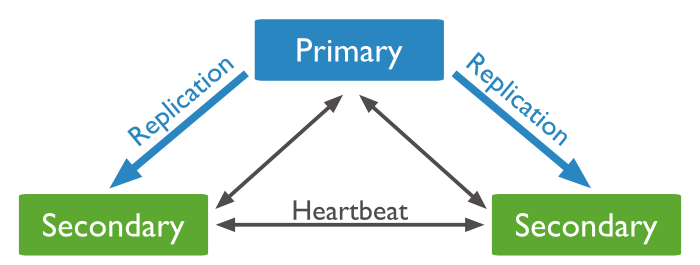
\includegraphics[width=0.40\textwidth]{img/mongodb-replica-set-primary-with-two-secondaries}}
	\hfill
	\subfigure[Een voorbeeld cluster voor productie met 2 mongos, 3 shards en 3 configuratie servers.]{\label{fig:mongodb-sharding} 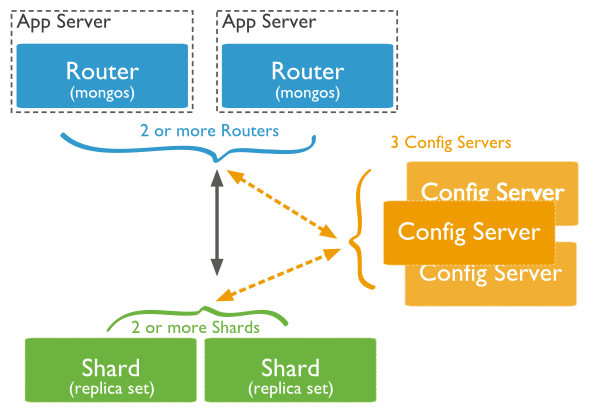
\includegraphics[width=0.50\textwidth]{img/mongo-sharded-cluster-production-architecture}}
	\caption{MongoDB Architectuur voor replicatie en datadistributie. Bron figuur \ref{fig:mongodb-replicaset}: \cite{mongodb-replicaset}, figuur \ref{fig:mongodb-sharding}: \cite{mongodb-shard}}
	\label{fig:mongodb-architectuur}
\end{figure}

\paragraph{Replicatie\cite{mongodb-replicaset}} Replicatie in MongoDB gebeurt door middel van een master/slave configuratie tussen verschillende \textbf{MongoD} instanties, of in hun termen primary/secondundaries. Deze instanties verkiezen zelf hun primary die verantwoordelijk is voor het afhandelen van de schrijfacties, de data zal vervolgens gerepliceerd worden naar de secundaries. Een verzameling van deze MongoD instanties wordt een \textit{replicaset} genoemd. Het is slechts mogelijk om een instantie tot een enkele set toe te voegen. De data is beschikbaar zo lang er meer dan de helft van de servers beschikbaar zijn. 

\paragraph{Data distributie\cite{mongodb-shard}} Horizontale schaalbaarheid wordt in MongoDB aangeboden door verschillende replicaset's of een enkele MongoD instantie te combineren tot een cluster. In het geval van de tweede keuze, zal de data niet gerepliceerd worden en wordt om deze reden niet aangeraden voor productie. 
\subparagraph{Shards} Sharding gebeurt automatisch op een collectie nadat is aangegeven dat men deze wilt verdelen over de gespecificeerde delen. Voor het uitvoeren van deze sharding zijn er nog 2 extra servers types nodig: configuratie servers en toegangsserver. 
\subparagraph{Configuratie servers} De configuratie servers slaan de meta data van de cluster op zoals de verschillende shardings. Deze configuratie set bestaat in productie uit exact 3 servers.
\subparagraph{Toegangsserver} De toegangsserver haalt de configuratie op uit de configuratie servers en biedt toegang voor de gebruiker aan tot de cluster. Er kunnen een onbepaald aantal toegangsservers zijn in cluster. 

De configuratie van de verschillende delen gebeurt op verschillende manieren. Bij replicatie krijgt elke set een naam die in de configuratiebestanden van elke configuratie wordt gezet, nadien wordt via één instantie de verschillende instanties toegevoegd via de API. Bij de cluster worden bij het opstarten van de toegangsservers de set van configuratieservers meegegeven, het opzetten van de verschillende shards gebeurt via een toegangsserver m.b.v. de API. 

\subsection{Pgpool-II (PostgreSQL)\cite{pgpool-doc}}
Pgpool-II kan op 4 verschillende manieren werken, in deze opstelling is er gekozen voor de replicatie mode omdat deze zowel replicatie, belastingsverdeling, failover en online recovery aanbiedt. Er is de mogelijkheid om ook data distributie aan te bieden maar dit is niet getest. 

Vervolgens zal de datastructuur en de architectuur besproken worden.  
\subsubsection{Datastructuur}
De data structuur en query mogelijkheden van Pgpool-II zijn gelijklopend aan deze van PostgreSQL. Net zoals in PostgreSQL bestaat het systeem uit een schema die verschillende databases kan bevatten. In een database zijn vervolgens verschillende tabellen die de records bevatten. Voor het opslaan van de data dient de volledige tabel met al de kolommen gespecificeerd zijn. 

Pgpool-II ondersteunt bijna de volledige query mogelijkheden die in de testen nodig zijn, er zijn enkele restricties die beschreven zijn op in de sectie \textit{Restrictions} van de documentatie\cite{pgpool-doc}. De query mogelijkheden zijn uitgebreid en ondersteunen naast de benodigde 5 queries, nog join acties. 

\subsubsection{Architectuur}
Een Pgpool-II infrastructuur bestaat uit 2 delen, een data niveau en een routing niveau, een overzicht is gegeven in figuur \ref{fig:Pgpool-structure}. 

\begin{figure}[h!]
\centering
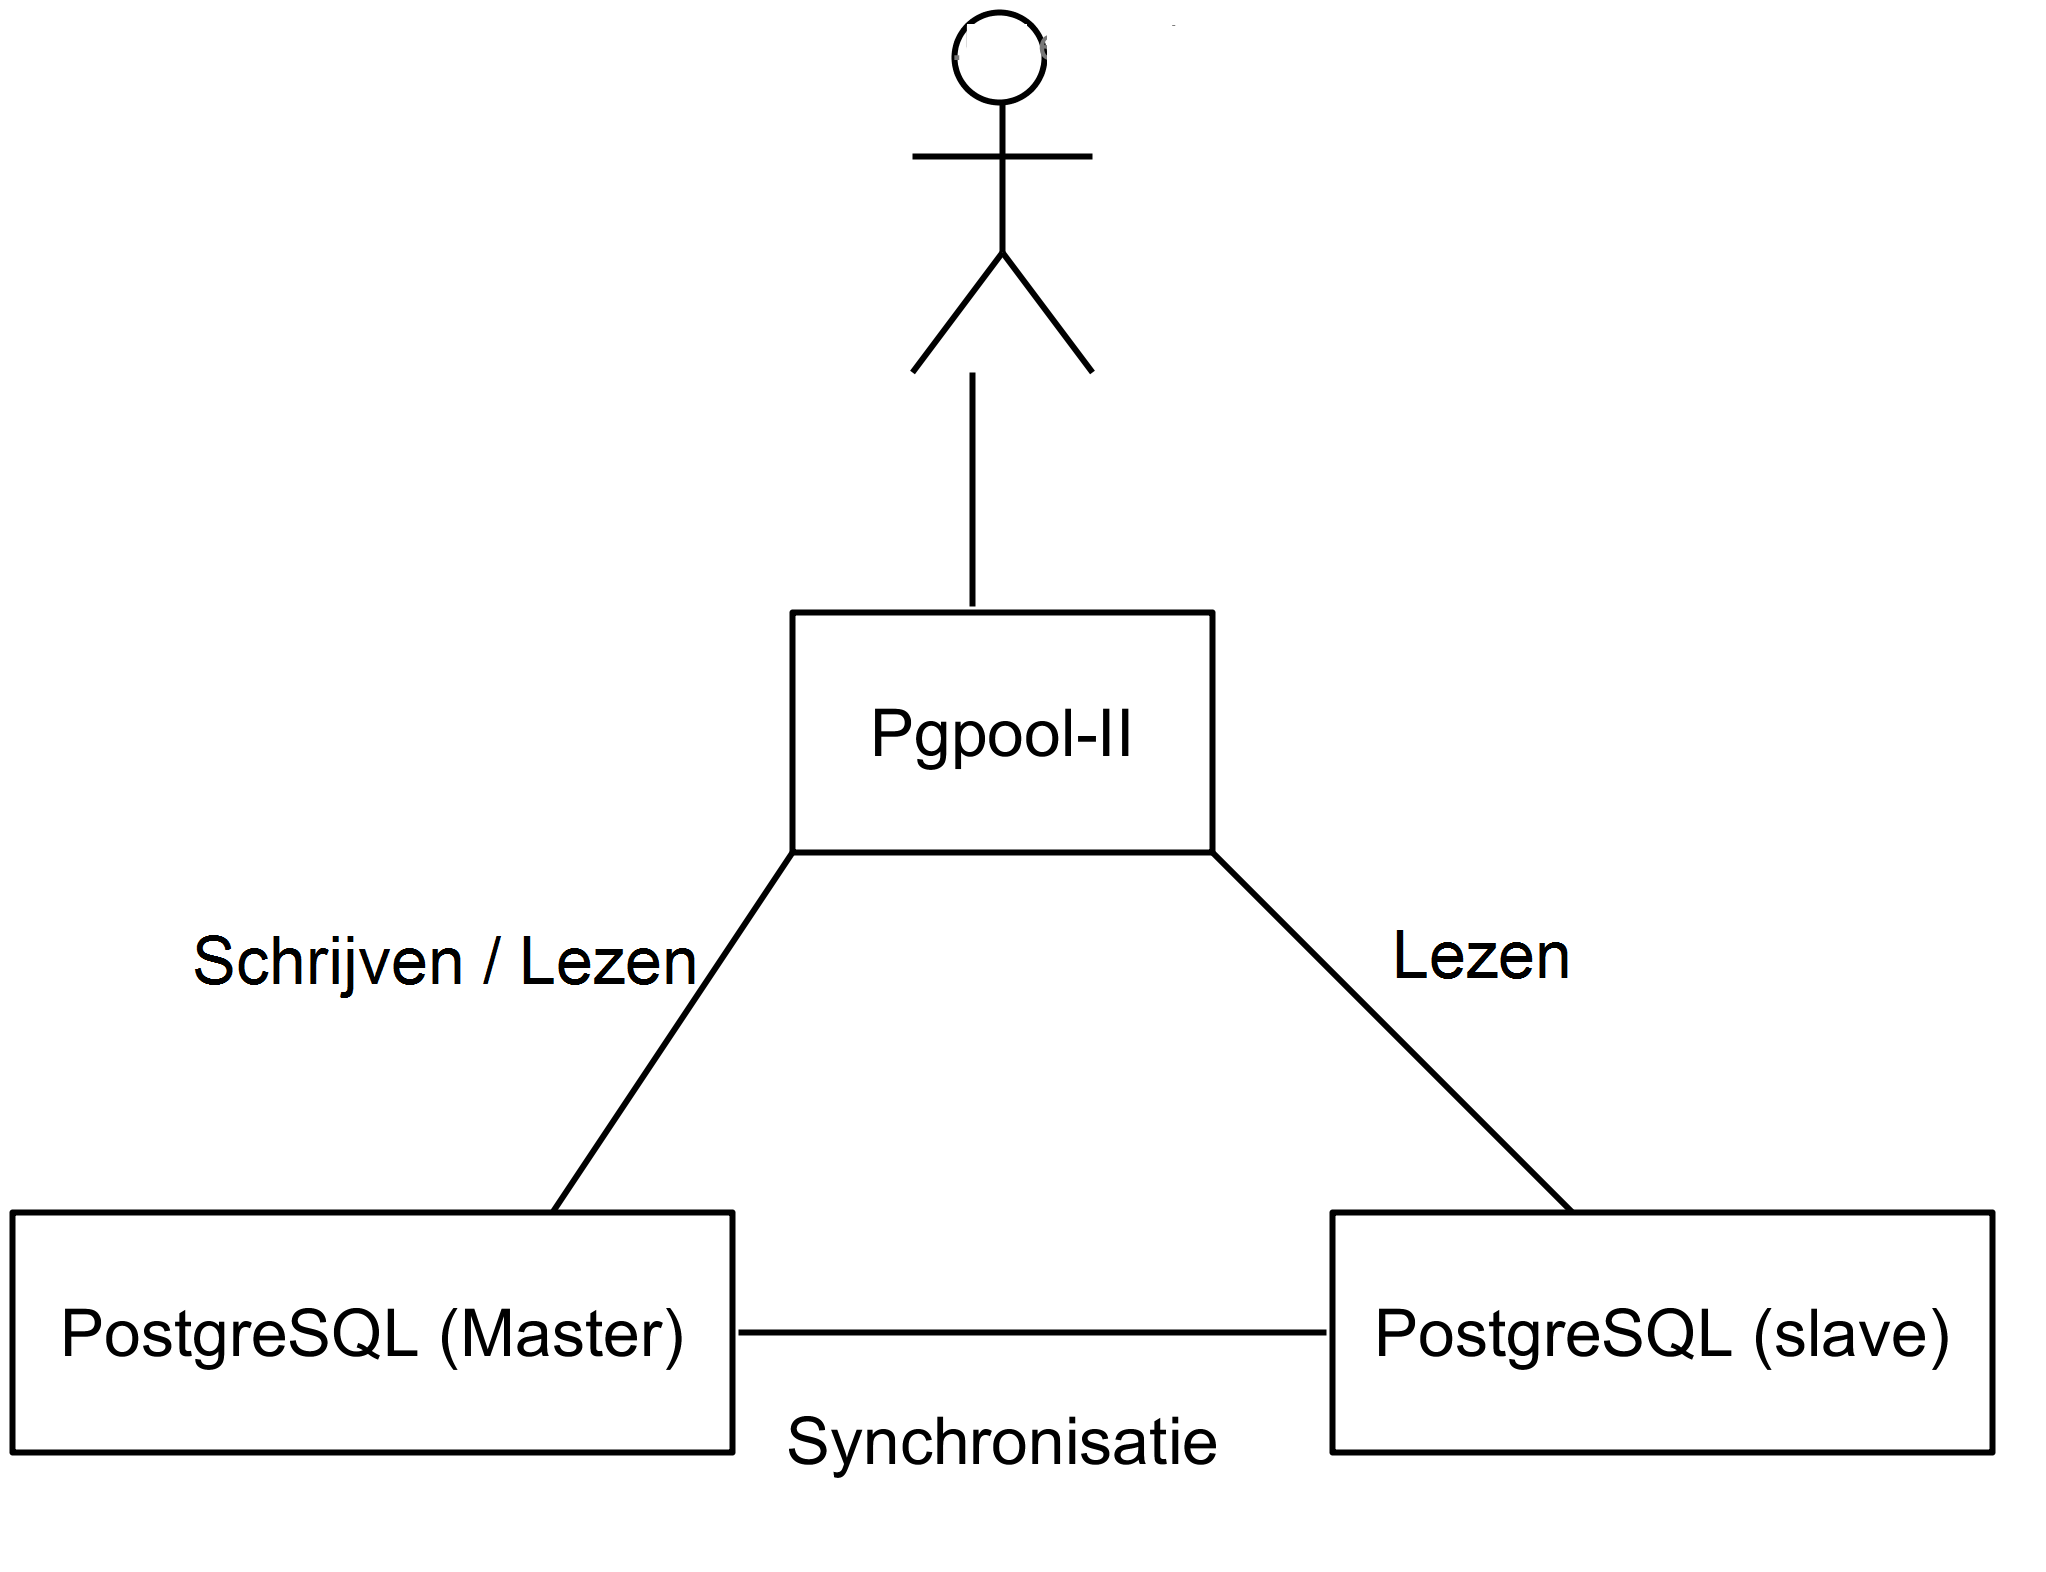
\includegraphics[width=0.5\linewidth]{img/Pgpool-structuur}
\caption{Systeemarchitectuur van Pgpool-II.}
\label{fig:Pgpool-structure}
\end{figure}

Op data niveau bestaat een individuele service uit een PostgreSQL installatie waarbij enkele extra functies en bestanden worden geïnstalleerd met een aanpassing aan de configuratie bestanden.  Daarnaast moet er voor de online recovery ook ssh toegang voorzien worden tot al de PostgreSQL servers. De verschillende data machines hebben een master/slave structuur waar al de schrijfacties naar de master worden gestuurd en de rest verdeeld over al de machines. De master doet aan synchronisatie met behulp van de \textit{Write-ahead-log} van PostgreSQL waar al de schrijfactie worden gelogd. 

Op routing niveau draait een Pgpool-II service die als management service dient, hij bepaalt wie master en slave is, volgt de status op van de data services en doet aan online recovery. Bij het aanmaken van een database connectie naar welke service de leesoperaties zullen gaan, zo wordt de leesbelasting verdeeld. 

Pgpool-II kan ook in de parallel mode werken zodat er de mogelijkheid is tot horizontale schaalbaarheid, ook is er de mogelijkheid om caching aan te zetten en een integratie met Memcache is ondersteund. 

\section{Selectie en uitwerking van de testsoftware}
De testen zijn geïmplementeerd als een uitbreiding van YCSB\cite{cooper2010benchmarking} omwille van verschillende redenen. Allereerst is de broncode publiek beschikbaar onder Apache 2.0, daarnaast is dit een uitgebreid systeem voor het uitvoeren van performantie benchmarking aan de hand van de vertraging op DBMS. Hierdoor heeft deze al een uitgebreide ondersteuning voor tal van systemen, waaronder al de gekozen systemen. Wel is deze ondersteuning zo veel mogelijk geoptimaliseerd voor de systemen zodat er maximaal gebruikt wordt van de functionaliteiten van het systeem, dit houdt in dat er bijvoorbeeld bij het opstellen van de range queries rekening gehouden wordt met het aantal records dat nodig is. 

De 2 testen, beschikbaarheidstest en consistentie test, worden op verschillende manieren geïmplementeerd. 

\paragraph{Beschikbaarheidstest} De beschikbaarheidstest wordt geïmplementeerd door middel van \gls{eventsupport}, hiermee kan er op vooraf gedefinieerde momenten een bepaald Unix commando uitgevoerd worden. De configuratie gebeurt met behulp van een XML bestand met de parameters van \ref{table:beschikbaarheidinput} die meegegeven wordt aan de parameter $eventFile$, de output komt in het logbestand met de elementen van tabel \ref{table:beschikbaarheidoutput}. 

Met behulp van deze uitbreiding zullen de beschikbaarheidstesten nadien uitgevoerd kunnen worden. Er zal gekeken worden naar de verandering in vertraging op een query waarmee kan bekeken worden of het systeem nog beschikbaar is. 

\begin{minipage}[b]{0.5\textwidth}
		\begin{tabular}{l|l}
			\textbf{Naam} & \textbf{eenheid} \\ 
			\hline ID & String \\ 
			Starttijdstip & milliseconden \\ 
			Commando & String \\ 
		\end{tabular} 
	\captionof{table}{Configuratie van event support}
	\label{table:beschikbaarheidinput}
\end{minipage}
\hfill
\begin{minipage}[b]{0.5\textwidth}

\begin{tabular}{l|l}
\textbf{Naam} & \textbf{eenheid} \\ 
\hline ID & String \\ 
Starttijdstip & milliseconden \\ 
Duur van de actie & microseconden \\
Gestart? & Boolean \\
Beëindigd? & Boolean \\
Exit code & Integer 
\end{tabular}
\captionof{table}{Uitvoer van event support}
\label{table:beschikbaarheidoutput}
\end{minipage}

\paragraph{Consistentie testen} Voor de consistentie testen is er een extra module geïmplementeerd die dit gedrag uitvoert. In deze uitwerking leest de schrijver niet zijn eigen data, al zou dit eenvoudig mee geïmplementeerd kunnen worden, dit is niet getest omdat het niet nodig was in deze testen. De testen kunnen uitgebreid geconfigureerd worden om enkel te testen wat nodig is: een overzicht van de configuratie parameters, uitgezonderd de locatie van de logbestanden, is te vinden in tabel \ref{table:consistentieinput}. Voor elke uitgevoerde query, wordt een record aangemaakt met de data van tabel \ref{table:consistentieuitvoer}. 

\begin{table}[t]
		\begin{tabular}{l|l|l}
			\textbf{Naam} & \textbf{eenheid} & \textbf{Omschrijving} \\ 
			\hline consistencyTest & Boolean & Het activeren van de consistentie test\\ 
			addSeparateWorkload & Boolean & Het toevoegen van een een extra belasting \\ 
			starttime & Milliseconden & Het moment dat de consistentie testen beginnen \\
			readThreads & Integer & Het aantal lees gebruikers \\ 
			consistencyDelayMillis & Milliseconden & Het interval waarin een lees gebruiker opnieuw het record leest \\ 
			newrequestperiodMillis & Milliseconden & Het interval waarin een schrijf gebruiker opnieuw een record schrijft \\ 
			readProportionConsistencyCheck & Float ($0\leq x \leq 1)$ & Het percentage van schrijfacties schrijven is \\ 
			updateProportionConsistencyCheck & Float ($0\leq x \leq 1)$ & Het percentage van schrijfacties updaten is \\ 
			stopOnFirstConsistency & Boolean & Stoppen zodra de eerste keer een correct record is gelezen \\ 
			maxDelayConsistencyBeforeDropInMicros & Microseconden & De maximale afwijking dat de eigenlijke start van de query mag hebben t.o.v. het geplande moment \\ 
			timeoutConsistencyBeforeDropInMicro & Microseconden & De maximale tijd dat een leesactie opnieuw geprobeerd wordt\\
		\end{tabular} 
	\captionof{table}{Configuratie van de consistentie testen}
	\label{table:consistentieinput}
\end{table}
\hfill


\begin{table}[t]
\centering
		\begin{tabular}{l|l|l}
			\textbf{Naam} & \textbf{eenheid} & \textbf{Omschrijving} \\ 
			\hline Tijd & Microseconden & Het moment dat de schrijfactie moest starten\\ 
			GebruikersID & R/W-Integer & Het id van de gebruiker (W-0, R-0, R-1, ..) \\ 
			Start & Microseconden & Het moment dat actie is begonnen \\
			Vertraging & Microseconden & De tijd dat de actie heeft geduurd \\ 
			Waarde & String & De gelezen of geschreven waarde \\ 
		\end{tabular} 
	\captionof{table}{Uitvoer van een enkel query in de consistentie testen}
	\label{table:consistentieuitvoer}
\end{table}

De code van deze testen is beschikbaar op GitHub in \url{https://github.com/thuys/ycsb} en te gebruiken onder Apache 2.0 licentie. \todo{Check}

\section{Installatie en opstelling van de DBMS's en YCSB}
Het uitvoeren van de testen vereist het opstellen van het volledige systeem en configuratie van de verschillende DBMS's. Voor het uitvoeren van de verschillende testen is het slechts nodig om het systeem een enkele keer op te zetten. Maar om de testen eenvoudiger te kunnen uitvoeren op verschillende infrastructuren en andere de resultaten te laten controleren, is de installatie en configuratie van het systeem geautomatiseerd. 

De automatisatie gebeurt met het Integrated configuration Management Platform (\gls{IMP}) beschreven in \cite{KULeuven-453199}. Dit modulair framework is uitgebreid met de 3 DBMS's en YCSB! waardoor de configuratie als een declaratief gewenste staat wordt uitgedrukt. \gls{IMP} zal deze staat toepassen op de verschillende systemen bij het uitrollen. 

Een uitgebreidere bespreking van de uitwerking in IMP kan gevonden worden in appendix \ref{app:IMP}. 

Voor de uitvoering van de testen, is er voor elk DBMS gekozen voor een minimaal aantal instantie die datadistributie én replicatie ondersteunt, voor de laatste eigenschap zou de data beschikbaar moeten zijn bij het uitvallen van 1 server. In de testen is er enkel gefocust op het uitvallen van dataservers, niet naar configuratieservers. Om deze reden zijn minimaal opgezet. 

De opstelling van de systemen is getoond in figuur \ref{fig:deployment-testomgeving}, elk van de systemen zal in meer detail besproken worden. Elk van de systemen wordt opgesteld op een machine waarvan er verschillende configuraties mogelijk zijn, voor een overzicht, zie tabel \ref{table:systeemconfiguraties}. 
\todo{Uitleggen wat Ephemeral Disk is}
\begin{table}[h!]
	\centering
	\begin{tabular}{l| l l l l}
	\textbf{Naam} & \textbf{Processor(s)} & \textbf{RAM} & \textbf{Harde schijf} & \textbf{Extra} \\
	\hline
	Normal.fs & 2 & 2GB &  10 GB & 30GB Ephemeral Disk \\ 
	Large & 2 & 4GB &  10 GB & \\
	Large.fs & 2 & 4GB &  10 GB & 50GB Ephemeral Disk\\
	\end{tabular}
	\caption{Overzicht mogelijke systeemconfiguraties}
	\label{table:systeemconfiguraties}
\end{table}

\paragraph{HBase} Voor HBase wordt de data standaard 3 maal gerepliceerd en zijn er voor datadistributie dus 4 data instanties nodig die elk een HBaseRegionServer en Hadoop datanode zijn. Verder is er nog de nood aan een HMaster (1 instantie), Zookeeper en Hadoop namenode (1 instantie). Dit brengt het totaal op 6 instanties. Een overzicht is getoond in figuur \ref{fig:HBase-deployment}. 

\paragraph{Pgpool-II} Bij Pgpool-II is er ondersteuning voor horizontale schaalbaarheid in de parallel mode maar dit is niet getest. Om deze reden is er enkel replicatie toegepast waarvoor er 3 instanties zijn: een Pgpool-II instantie en twee PostgreSQL instanties. Een overzicht is getoond in figuur \ref{fig:pgpool-deployment}. 

\paragraph{MongoDB} MongoDB heeft ondersteuning in replicatie en datadistributie. Voor het beschikbaar zijn van de data bij het uitzetten van een enkele instantie, zijn er 3 MongoDB datanodes nodig in een replicaset. De data wordt verdeeld over 2 replicaset met behulp van sharding. Omdat de toegangsserver en configuratie instanties niet veel resources innemen, zijn deze verspreid over de verschillende data instanties. Om deze reden zijn er in totaal 6 instanties nodig. Deze zijn beschreven in \ref{fig:MongoDB-deployment}. \todo{Check dat het er 6 zijn!}

\paragraph{YCSB!} YCSB! kan naar meerdere instanties uitgerold worden. Bij de calibratietesten zullen er 2 instanties gebruikt worden, maar er zal blijken dat dit niet een limiterende factor is. Voor het uitvoeren van de eigenlijke testen, zal er gebruik gemaakt worden van een enkele YCSB! instantie, namelijk VM-1.  Een overzicht is getoond in figuur \ref{fig:YCSB-deployment}. 

\begin{figure}[h!]
\centering
\subfigure[Deployment van HBase met 6 instanties. ]{\label{fig:HBase-deployment}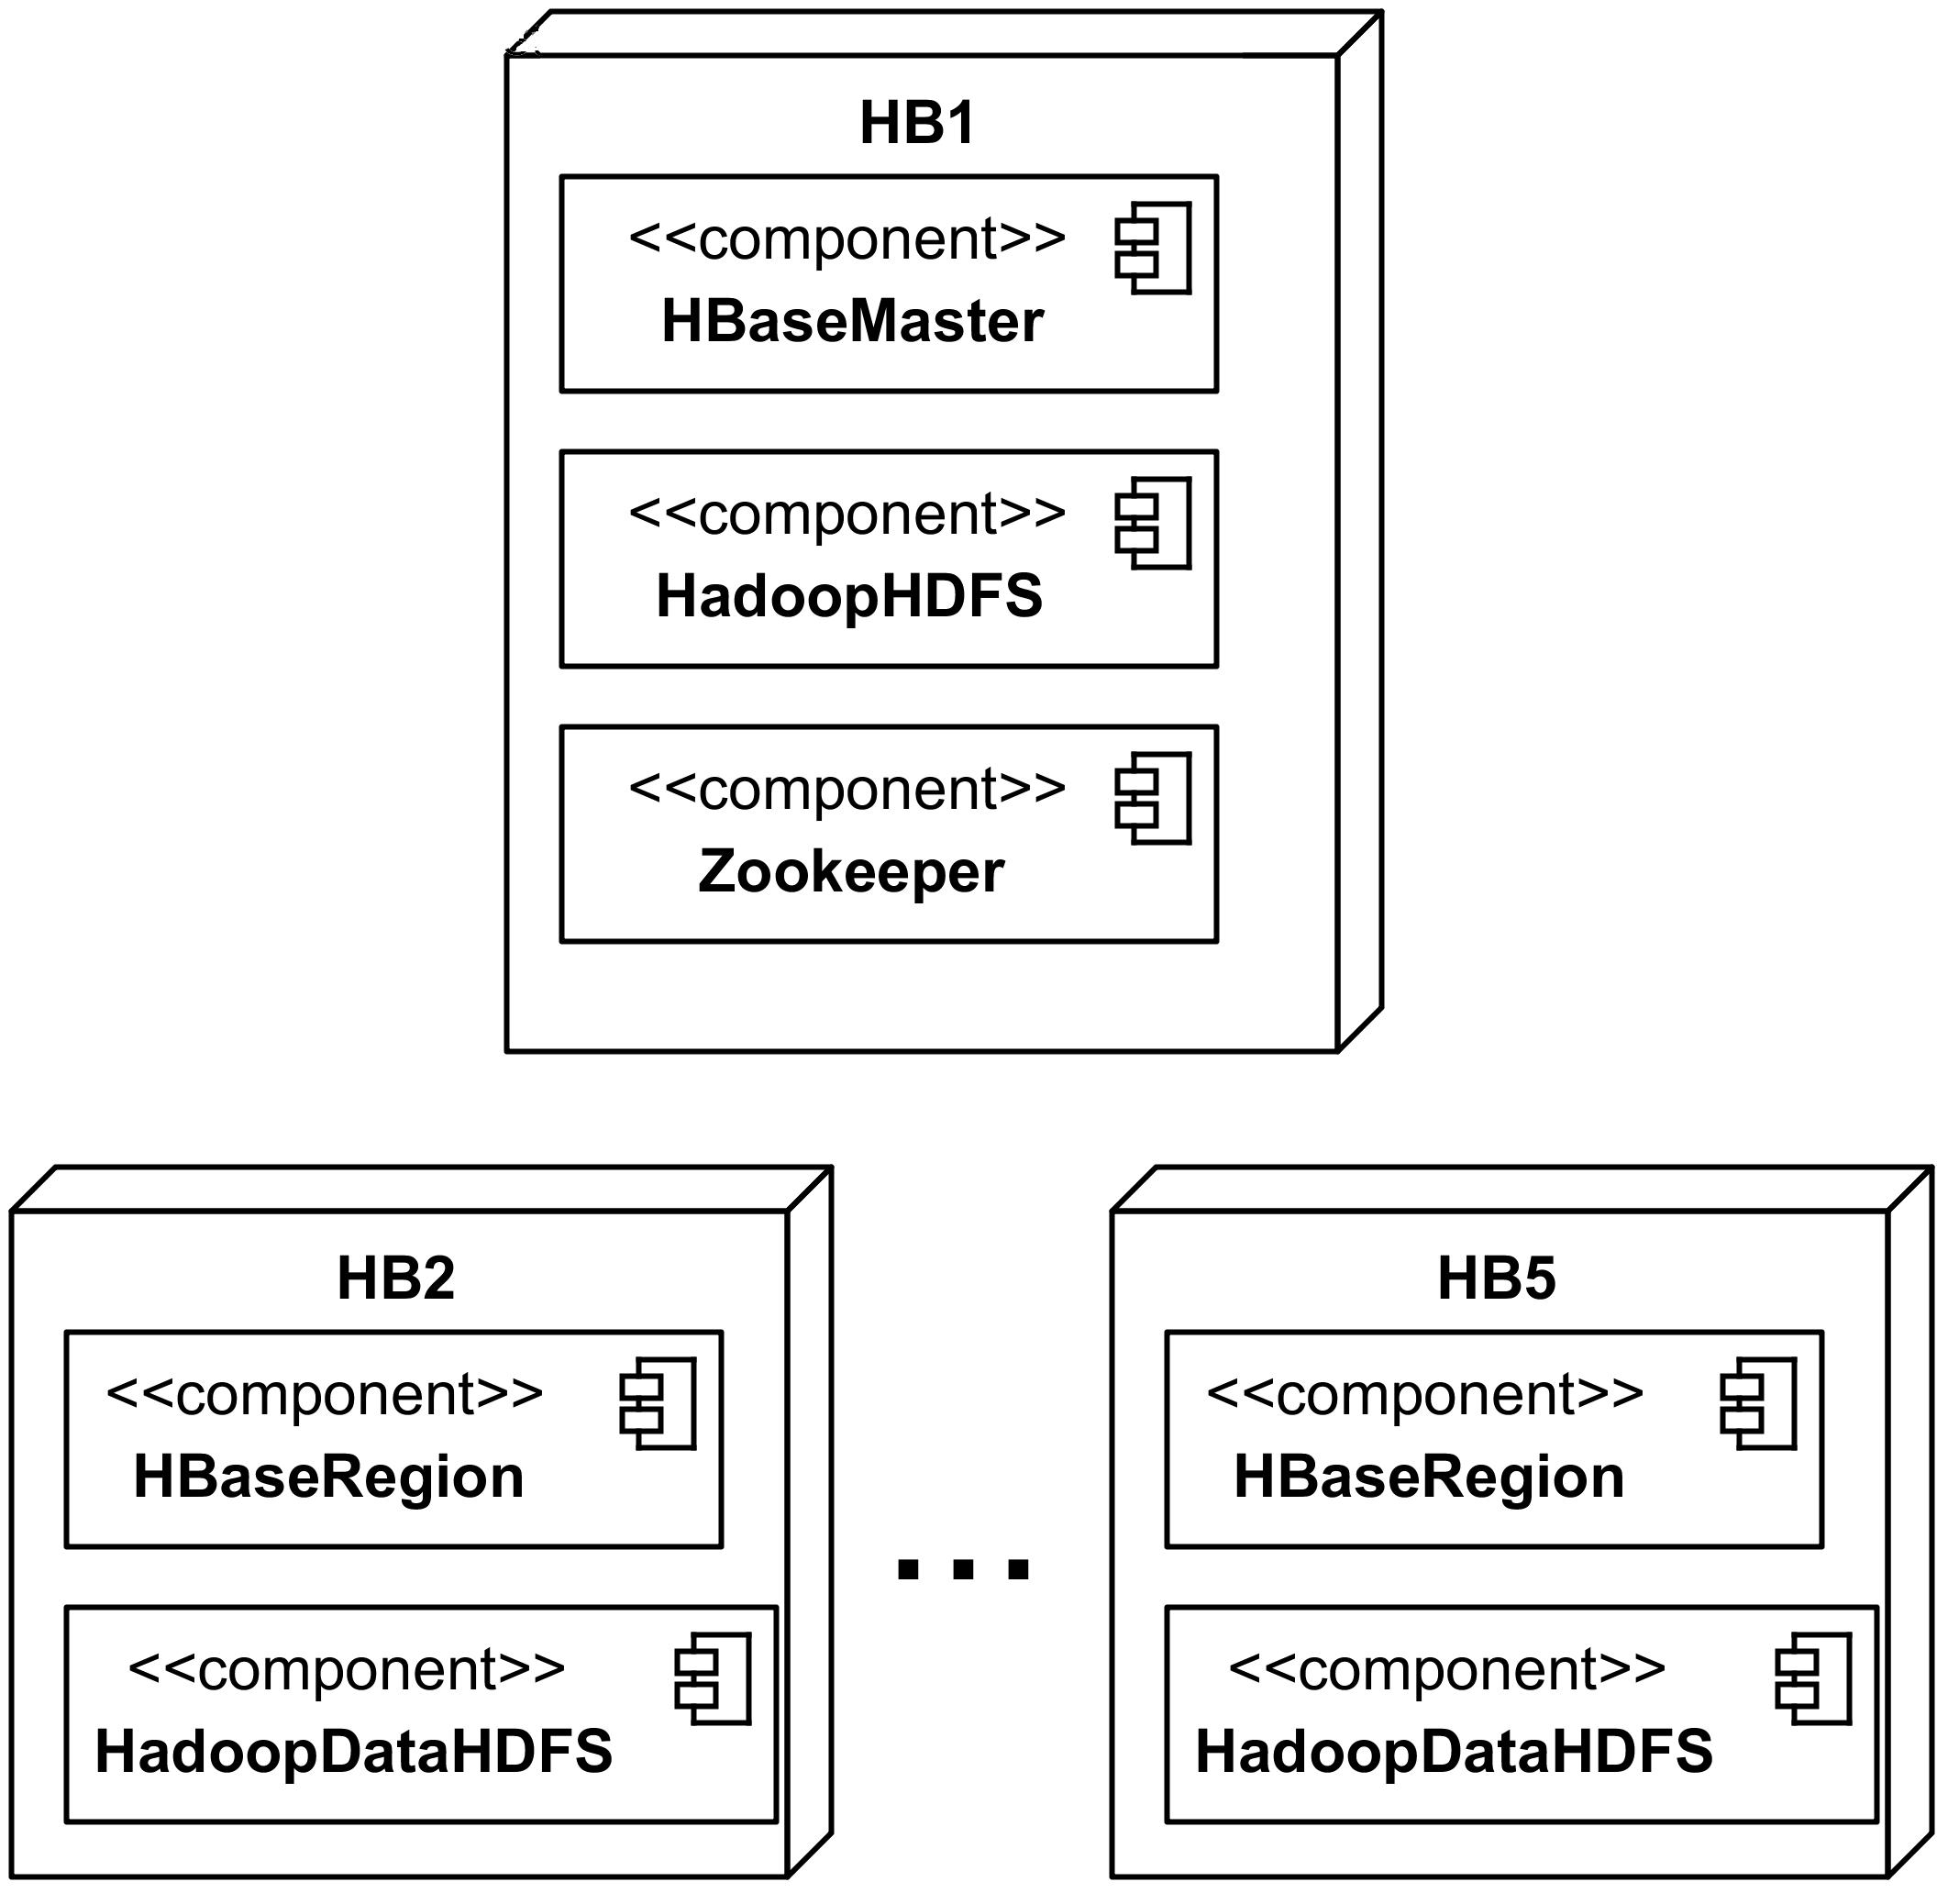
\includegraphics[width=0.55\textwidth]{img/HBase-deployment}}
\subfigure[Deployment van Pgpool-II met 3 instanties. ]{\label{fig:pgpool-deployment}\includegraphics[width=0.35\textwidth]{img/Pgpool-II-deployment}}
\subfigure[Deployment van MongoDB met 5 instanties. ]{\label{fig:MongoDB-deployment}\includegraphics[width=0.65\textwidth]{img/MongoDB-deployment}}
\subfigure[Deployment van de testomgeving met 2 YCSB instanties. ]{\label{fig:YCSB-deployment}\includegraphics[width=0.25\textwidth]{img/YCSB-deployment}}
\caption{Deployment van de verschillende DBMS's en de testomgeving.}\label{fig:deployment-testomgeving}
\end{figure}


\section{Uitvoeren van de calibratie en testen}
Voor het uitvoeren van de volledige benchmarking dient eerst de verdeling van de type queries gespecificeerd worden, deze zijn voor alle verschillende systemen gelijk. Een overzicht van deze parameters kunnen gevonden worden in tabel \ref{table:calibratiequeries}. \todo{Verklaring toevoegen} 

\paragraph{Calibratie testen} Voor de calibratie van de omgeving zijn er 2 soorten testen gedraaid, de parameters voor het aantal connecties kunnen gevonden worden in tabel \ref{table:calibratiegebruikers}. De parameters voor het aantal queries per second zijn te vinden in tabel \ref{table:calibratiequeriesperseconde}, in dit geval is het aantal gebruikers afhankelijk van de vorige test. 

\begin{table}[h!]
	\centering
	\begin{tabular}{l| l }
	\textbf{Naam} & \textbf{Waarde} \\
	\hline
	Aantal velden & 10 (1 key veld) \\
	Record grootte & 1KB (100byte/veld) \\
	Lees alle velden & true \\
	Invoeg queries (\textit{insert}) & 20\%\\
	Lees queries (\textit{select}) & 40\%\\
	Aanpas queries (\textit{update}) & 20\%\\
	Range queries (\textit{scan}) & 20\%\\
	Opvraag verdeling & zipfian (\textit{bepaalde records worden} \\
	& \textit{veel gelezen, andere weinig}) \\
	Maximale range grootte & 100 \\
	Verdeling range grootte & uniform \\
	\end{tabular}
	\caption{Overzicht van de query parameters}
	\label{table:calibratiequeries}
\end{table}

\begin{table}[h!]
	\centering
	\begin{tabular}{l| l}
	\textbf{Naam} & \textbf{Waarde}  \\
	\hline
	Ingeladen records  & 300 000 \\
	Pauze & 50s \\
	Executie tijd & 600s \\
	Aantal gebruikers & 1, 2, 3, 4, 5, 7, 10, 15, \\
	& 20, 30, 40, 50, 75, 100\\
	\end{tabular}
	\caption{Calibratie: Overzicht van de parameters voor het testen van het aantal gebruikers}
	\label{table:calibratiegebruikers}
\end{table}

\begin{table}[h!]
	\centering
	\begin{tabular}{l| l l }
		\textbf{Naam} & \multicolumn{2}{c}{\textbf{Waarde}}  \\
		
		& \textbf{HBase en MongoDB} & \textbf{Pgpool-II} \\
		\hline
		Ingeladen records  & 300 000 & 300 000 \\
		Pauze & 50s & 50s \\
		Executie tijd & 600s & 600s\\
		Theoretisch aantal records  & 50, 100, 200, 300,   & 20, 50, 100, 150,   \\
		per seconde & 400, 500, 600, 700, & 200, 250, 300, 400,  \\
		& 800, 900, 1000, 1500,  & 500, 600, 700, 800,  \\
		& 2000, 3000, 4000 &  900, 1000 \\
	\end{tabular}
	\caption{Calibratie: Overzicht van de parameters voor het testen van het aantal records per seconde}
	\label{table:calibratiequeriesperseconde}
\end{table}

\paragraph{Beschikbaarheidstesten} Bij het uitvoeren van de testen op beschikbaarheid van de verschillende systemen zijn de parameters in tabel \ref{table:beschikbaarheidstesten-parameters} gebruikt. De commando's voor het stoppen en starten van de systemen zijn te vinden in tabel \ref{table:beschikbaarheidstesten-commandos}.  Voor Pgpool-II is er een extra commando toegevoegd dat na het herstarten van de systemen wordt uitgevoerd, dit komt omdat er geen automatische recovery in Pgpool-II is. Tenslotte worden deze testen uitgevoerd op al de datanodes, een overzicht hiervan met de overeenkomstige service is te vinden in tabel \ref{table:beschikbaarheidstesten-nodes}.

\begin{table}[h!]
	\centering
	\begin{tabular}{l| l }
		\textbf{Naam} & \textbf{Waarde}  \\
		\hline
		Ingeladen records  & 300 000 \\
		Pauze & 50s \\
		Executie tijd & 900s \\
		Stoppen & Op 300s \\
		Starten & Op 600s \\
	\end{tabular}
	\caption{Beschikbaarheidstesten: Overzicht van de parameters}
	\label{table:beschikbaarheidstesten-parameters}
\end{table}
\begin{table}[t]
	\centering
		\begin{tabular}{l|l}
			\multicolumn{2}{c}{\textbf{Stoppen}} \\
			\textbf{Wat} & \textbf{Commando} \\ 
			\hline
			Zachte stop & service \{\{service-name\}\} stop \\ 
			Harde stop & kill -KILL \{\{process Id\}\} \\ 
			Netwerk onderbreken & iptables -A OUTPUT -d 0.0.0.0/0 -j DROP  \\ 
			\multicolumn{2}{c}{} \\
			\multicolumn{2}{c}{\textbf{Heropstarten}} \\
			\textbf{Wat} & \textbf{Commando} \\ 
			\hline
			Zachte start & service \{\{service-name\}\} restart \\ 
			Harde start & service \{\{service-name\}\} restart \\ 
			Netwerk herstellen & iptables -D OUTPUT 1  \\ 
			\multicolumn{2}{c}{} \\
			\multicolumn{2}{c}{\textbf{Speciale commando's}} \\
			\textbf{Wat} & \textbf{Commando} \\ 
			\hline
			Pgpool-II & /usr/local/bin/pcp\_recovery\_node -d 10 \{\{pgpool host\}\} \{\{port\}\} \\
			\hspace*{0.5cm} (Online recovery) &  \hspace*{0.5cm} \{\{gebruikersnaam\}\} \{\{wachtwoord\}\}  \{\{node nummer\}\} \\
		\end{tabular} 
	\captionof{table}{Beschikbaarheidstesten: Overzicht van de commando's voor het stoppen en starten in de verschillende modes. }
	\label{table:beschikbaarheidstesten-commandos}
\end{table}

\begin{table}[h!]
	\centering
	\begin{tabular}{l| l l }
		\textbf{Naam} & \textbf{Instanties} & \textbf{Service naam} \\
		\hline
		\multirow{2}{*}{HBase}  & \multirow{2}{*}{HB3, HB4, HB5, HB6} & hbase-regionserver \\
		& & hadoop-hdfs-datanode \\
		\multirow{2}{*}{MongoDB}  & MDB1, MDB2, MDB3, & \multirow{2}{*}{mongodb-dataserver}\\
		& MDB4, MDB5, MDB6 & \\
		Pgpool-II  & PG1, PG2 & postgresql \\
	\end{tabular}
	\caption{Beschikbaarheidstesten: Overzicht van de instanties naar figuur \ref{fig:deployment-testomgeving}}
	\label{table:beschikbaarheidstesten-nodes}
\end{table}\todo{Check of het er nu echt 6 zijn}

\paragraph{Consistentie testen} Voor de consistentie testen moeten de parameters van tabel \ref{table:consistentieinput} geconfigureerd worden, de parameters zijn te vinden in tabel \ref{table:consistentie-testen-parameters}. Deze test wordt uitgevoerd op HBase en MongoDB, om de analyse van de gegevens eenvoudiger te maken is er bij MongoDB gekozen om de test enkel uit te voeren op een replicaset en niet op een volledige cluster. Er is een aanname gedaan dat het consistentie venster bepaald is door de tijd dat het duurt dat de gegevens beschikbaar zijn op al de verschillende instanties van een replicaset, het testen van een cluster voegt zo extra complexiteit toe. Deze test zou in de toekomst ook uitgevoerd kunnen worden op een cluster maar is in dit geval niet gedaan.  

\begin{table}[t]
	\centering
		\begin{tabular}{l|l}
			\textbf{Naam} & \textbf{Waarde} \\ \hline
			Ingeladen records  & 300 000 \\
			Pauze & 50s \\
			Executie tijd & 900s \\	
			starttime & 10s \\
			readThreads & 30 \\ 
			consistencyDelayMillis & 60ms \\ 
			newrequestperiodMillis & 500ms \\ 
			readProportionConsistencyCheck & 50\% \\ 
			updateProportionConsistencyCheck & 50\% \\ 
			stopOnFirstConsistency & True \\ 
			maxDelayConsistencyBeforeDropInMicros & 300ms \\ 
			timeoutConsistencyBeforeDropInMicro & 300ms \\
		\end{tabular} 
	\captionof{table}{Consistentie testen: Overzicht van de parameters}
	\label{table:consistentie-testen-parameters}
\end{table}

\section{Verzamelen en analyse van de testresultaten}
\todo{Te schrijven}


